In this chapter we present two algorithms for performing Einstein summation. First,
we introduce our implementation of the four mapping rules developed in ``Efficient and Portable
Einstein Summation in SQL"~\cite{sql_einsum}, to generate SQL queries for solving Einsum problems.
This will serve as a baseline to compare other algorithms against. Second, we explain our C++
implementations with multiple levels of optimization. The underlying algorithm of the C++
implementations builds on Torch's strategy of mapping Einsum operations to a batch matrix
multiplication kernel. Both algorithms, namely the algorithm for the SQL implementation and
the algorithm used for the C++ versions, decompose large Einstein summation operations
into smaller, pairwise operations to exploit efficient contraction paths.

\section{The SQL Algorithm}
In this section, we present Blacher et al.'s~\cite{sql_einsum} algorithm and our
implementation of it for mapping format strings and the corresponding tensors to SQL,
enabling Einstein summation in databases. First, we introduce the portable schema for
representing tensors, specifically sparse tensors, in SQL. We then show their four mapping
rules to generate non-nested Einsum queries from arbitrary format strings. Next, we
explain how we exploit efficient contraction paths by decomposing large Einsum queries
into smaller parts. Finally, we present implementation details of the SQL algorithm.

\subsection{Portable Schema for Tensors}
Blacher et al. chose the COO format to represent tensors as it only uses integers and
floating point numbers, which results in a vendor independent schema for encoding tensors
across various database management systems (DBMS). For example, a 3D tensor $A \in
    \mathbb{R}^{I \times J \times K}$ has the following schema:

\[
    A(i\ \ INT,\ \ j\ \ INT,\ \ k\ \ INT,\ \ val\ \ DOUBLE)
\]
%
Each tensor is stored in a separate table. In the example, table A stores a 3D tensor,
where each value ($val$) can be addressed by specifying the corresponding indices
($i$,~$j$,~$k$).

\subsection{Mapping Einstein Summation to SQL}
\label{subsec:sql:rules}
``Efficient and Portable Einstein Summation in SQL" introduces four rules for mapping
any tensor expression in Einstein notation to SQL.

\begin{description}[leftmargin=!,labelwidth=\widthof{\bfseries R1}]
    \item [R1] All input tensors are enumerated in the FROM clause.
    \item [R2] The indices of the output tensor are enumerated in the SELECT clause
          and the GROUP BY clause.
    \item [R3] The new value is the SUM of all values multiplied together.
    \item [R4] Indices that are the same among input tensors are transitively equated
          in the WHERE clause.
\end{description}
%
Say we want to map the tensor operation given by $ik,k \rightarrow i$, a matrix-vector
multiplication, with tensors $A \in \mathbb{R}^{I \times K}$, $v \in \mathbb{R}^{K}$ and

\begin{equation*}
    A =
    \begin{bmatrix}
        0.0 & 1.0 \\
        0.0 & 0.0 \\
        5.0 & 0.0 \\
        0.0 & 0.0
    \end{bmatrix},
    \quad
    v =
    \begin{bmatrix}
        4.0 \\
        1.0
    \end{bmatrix}.
\end{equation*}
%
When applying all four rules to map the example tensor expression to SQL, we get the result
seen in Listing \ref{lst:einsum:sql}.

\begin{lstlisting}[caption={Einstein summation in SQL.}, captionpos={t}, label={lst:einsum:sql}]
    WITH A(i, j, val) AS (                          -- matrix A
        VALUES (0, 1, 1.0), (2, 0, 5.0)
    ), v(i, val) AS (                               -- vector v
        VALUES (0, 4.0), (1, 1.0)
    ) SELECT A.i AS i,                              -- R2
        SUM(A.val * v.val) AS val                   -- R3
      FROM A, v                                     -- R1
      WHERE A.j=v.i                                 -- R4
      GROUP BY A.i                                  -- R2
\end{lstlisting}
%
While all four rules are needed to ensure every possible Einstein summation problem
can be translated to SQL, for some tensor expressions the conditions to apply the rules
R2 and/or R4 are not fulfilled. If there are no indices after the arrow in the format
string, the output is scalar and does not require R2. Furthermore, if there are no common
indices among the input tensors, there is no summation in the tensor expression and R4
can be omitted. The rules guarantee a correct mapping, not a mapping with minimal code size.
In some cases, with additional checks, the SQL queries could be further simplified.

\subsection{Optimizing Contraction Order}
Mapping a tensor expression directly into a single, non-nested SQL query in Einstein
notation is known to produce execution times that are far from optimal, especially for operations
involving many tensors. The inefficiency stems from the fact that conventional query optimizers
are unaware of the contraction order of the repeating indices within tensor expressions and are
therefore incapable of effectively breaking down the query into smaller parts to exploit efficient
contraction paths as described in Section \ref{sec:tensor:contractions}.\\
One can get around this using intermediate tensors via subqueries or common table expressions,
which decomposes one large Einstein summation query into smaller pieces and lets the database
engine follow a pre-defined contraction order. More precisely, using GROUP BY and SUM
aggregation in intermediate computations enforces query engines to evaluate the query in the
right order.

% TODO: Edit this section to list the right arguments for calling sql_einsum_query()
\section{Implementation Details}
We implemented the algorithm for mapping Einsum format strings to SQL queries proposed by Blacher
et al. in Python 3.11.0 as a small package, only requiring Numpy as a dependency. When
calling \textit{sql\_einsum\_query()}, an Einsum notation string, the tensor names, and the tensor
data have to be supplied. The path argument is optional. When not supplied with a path, an
optimized contraction path is calculated using cgreedy~\cite{cgreedy}. The cgreedy package
provides a greedy algorithm approach for finding an efficient contraction order for any given
format string and associated tensors, utilizing multiple cost functions. The construction of the
query is separated into two parts. The first part creates the tensors in COO format as SQL
compatible structures and returns the appropriate query. The second part applies the decomposition
schema, more precisely, it uses either the supplied or the calculated contraction path to build a
contraction list. The entries of the contraction list dictate the order and the exact pairwise
operations necessary to solve the Einstein summation problem. These subproblems are also specified
in Einstein notation. To build the second part of the query, we iterate the contraction list and
apply the four mapping rules from Subsection \ref{subsec:sql:rules} to assemble the correct SQL
strings for the given pairwise contractions. Finally, we merge the two generated query parts and
return the complete query.

\section{The C++ Algorithm}
Our method expands on Torch's strategy of mapping the Einstein summation problems to batch matrix
multiplication (BMM). We give an overview of our approach that pre-processes tensors for pairwise
operations, calculates the result via a sparse BMM and finally post-processes the result to fit the
expected output format.

\subsection{Pre-Processing}
The pre-processing phase of the algorithm is critical for aligning the tensors in Coordinate List
(COO) format with the requirements of batch matrix multiplication. In order to achieve predictable
computations with the BMM, we apply the template seen in Figure \ref{fig:bmm:template}. The indices
of the two input tensors are grouped as follows:

% TODO: Right tensor index s_l is wrong in the figure. Change it to s_r.
\begin{figure}[H]
    \centering
    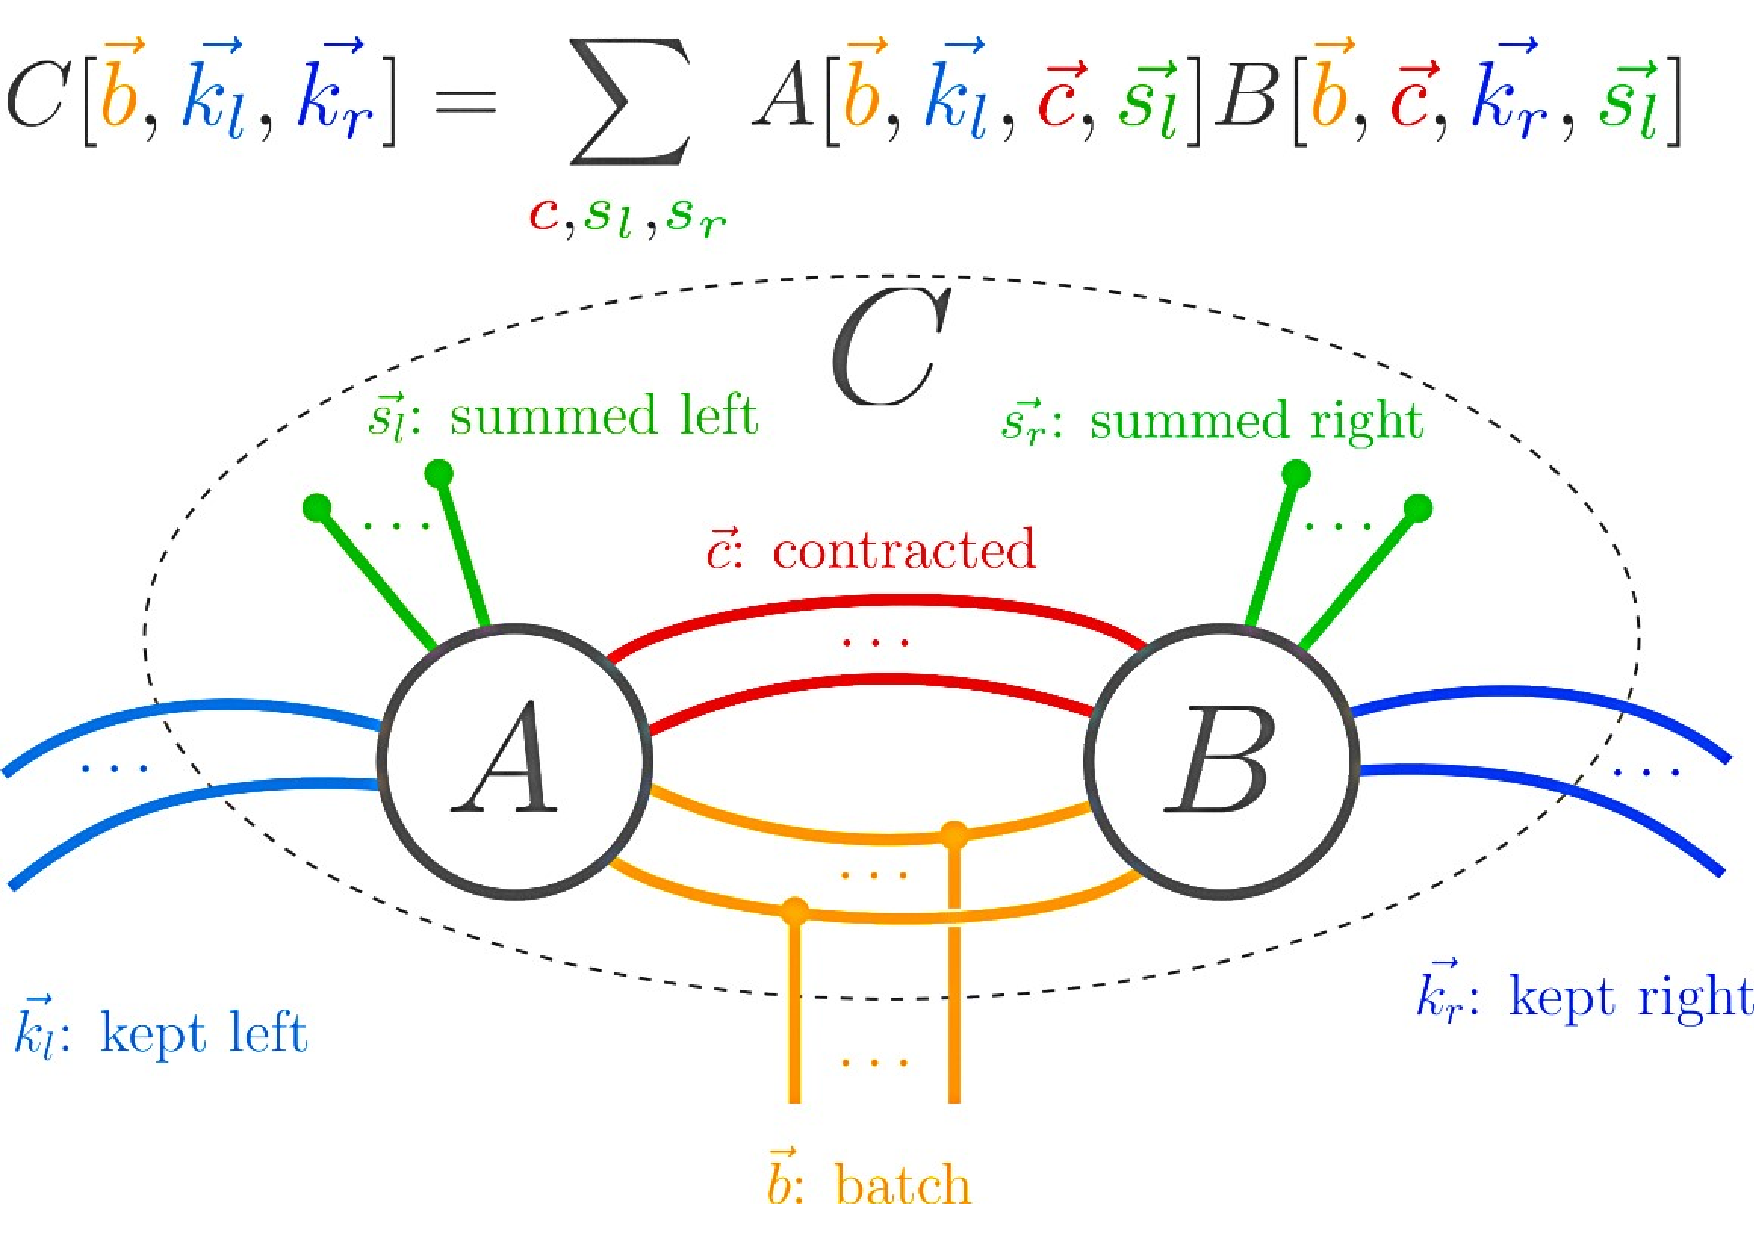
\includegraphics[scale=0.45]{gray_bmm_indice_grouping1_edited.pdf}
    \caption{The figure used by Gray J. \cite{jcmgray}  to describe the classification of indices
        used for the grouping. The left tensor has the index order $(b, k_l, c, s_l)$ and the right
        tensor $(b, c, k_r, s_r)$.}
    \label{fig:bmm:template}
\end{figure}
%
\begin{description}[leftmargin=!,labelwidth=\widthof{\bfseries Contracted Indices (c)}]
    \item [Batch Indices (b)] All individual batch dimensions have to be combined into a single
          batch dimension.
    \item [Contracted Indices (c)] The dimensions over which the contraction takes place.
    \item [Summed Indices (s)] All indices that only have a single occurence. This is grouped for
          both input tensors separately.
    \item [Kept Indices (k)] All indices and their dimensions that occur in only a single input
          tensor and in the output. This is grouped for both input tensors separately.
\end{description}
%
For our implementation we treat the removal of the summed indices as part of the pre-processing.
This means the input tensors for the BMM only have index order $(b, k_l, c)$ for the left term and
$(b, c, k_r)$ for the right term. For the COO format, since every index results in a column,
the index order translates to the columns, followed by a last column for the value. To enable the use
of this format we apply multiple pre-processing steps. First, the algorithm calculates appropriate
format strings for the COO tensors. The format strings should align with the requirements of the BMM
to ensure correctness and efficiency of the subsequent operation.\\
Besides computing the format strings, the algorithm computes the new shapes for the tensors.
In doing so, this step will combine all batch, contracted and kept dimensions into one single dimension
respectively and ignore dimensions not present in the format string. Precise computation of these new
shapes is critical to ensure that the tensors are aligned correctly for the BMM.\\
The computed format strings are used to call a special, single Einsum function. This function performs
Einstein summation on a single tensor, allowing for the computation of diagonals, summation over
specified dimensions and the permutation thereof. The new shapes are used to reshape the tensors to
comply with the dimensional requirements of BMM. Both of these steps are only performed if necessary.
The pre-processing will result in a COO tensor, which is suited for batch matrix multiplication.

\subsection{Sparse BMM}
The BMM computes the results in batches. In our case a batch only contains two elements. A COO tensors
rows with the same batch index represent a two dimensional matrix in COO format. A batch contains
the two matrices, one for each tensor, where the batch index is the same. Since the batch index of
the matrices in a batch are the same and we compute the products within batches, we represent them
without the batch index after selecting a batch. Say $A$ and $B$ are tensors with indices $(b, k_l, c)$
for $A$ and indices $(b, c, k_r)$ for $B$. The multiplication for the COO tensors is performed
using the following algorithm:

\begin{enumerate}[label*=\arabic*.]
    \item Get batches by interpreting rows of tensor A and B with the same batch index as COO matrices
          $A'$ and $B'$. For each batch perform the following operations:
    \item Transpose $B'$ by swapping columns $c$ and $k_r$ and sorting the rows of $B'$ by comparing
          column $k_r$'s entries followed by $c$'s entries.
    \item Let a row of $A'$ be represented as:
          \begin{equation*}
              \begin{bmatrix}
                  k_l^i & c^i & v^i \\
              \end{bmatrix}
          \end{equation*}
          and a row of $B'$ as:
          \begin{equation*}
              \begin{bmatrix}
                  k_r^j & c^j & v^j \\
              \end{bmatrix}
          \end{equation*}
          where $i$ and $j$ are the row indices, and $v^i$ and $v^j$ are the corresponding values.
          For example, as shown in Figure \ref{fig:bmm:algorithm}, for $i=3$ and $j=2$ the rows are:
          \begin{equation*}
              A':
              \begin{bmatrix}
                  1 & 3 & 1.89 \\
              \end{bmatrix}
              , B':
              \begin{bmatrix}
                  1 & 3 & 0.14 \\
              \end{bmatrix}
          \end{equation*}
          Now, iterate through the rows of $A'$ and $B'$. If $c^i = c^j$, compute and store:
          \begin{equation*}
              \begin{bmatrix}
                  k_l & k_r & v^i \cdot v^j \\
              \end{bmatrix}
          \end{equation*}
    \item If there are duplicate indices in the resulting matrix, sum their values and store the result.
    \item Sort the rows of the resulting matrix first by column $k_l$ and then by $k_r$.
    \item Append the resulting COO matrix to the final tensor $C$ with its batch index added as the
          first column $[b, k_l, k_r, v]$
    \item Repeat from 2. with next batch until all batches are done.
\end{enumerate}
The final tensor is returned and can now be post-processed.

% \mathbin{\color{blue}0}
\begin{figure}[H]
    \begin{alignat*}{5}
         & Steps \quad &              &                &                                                                                      &                                                                                                       &  &  &  & \\
         & 1.          &              & A(b, k_l, c)   &                                                                                      & = \begin{bmatrix}
                                                                                                                                                      b & k_l & c & v    \\
                                                                                                                                                      0 & 0   & 0 & 2.37 \\
                                                                                                                                                      0 & 0   & 1 & 0.45 \\
                                                                                                                                                      0 & 1   & 2 & 0.63 \\
                                                                                                                                                      0 & 1   & 3 & 1.89 \\
                                                                                                                                                      1 & 0   & 0 & 1.13 \\
                                                                                                                                                      1 & 0   & 1 & 0.08 \\
                                                                                                                                                  \end{bmatrix} \qquad
         &             & B(b, c, k_r) &                & = \begin{bmatrix}
                                                               b & c & k_r & v    \\
                                                               0 & 0 & 0   & 0.32 \\
                                                               0 & 0 & 2   & 2.57 \\
                                                               0 & 1 & 0   & 1.45 \\
                                                               0 & 3 & 1   & 0.14 \\
                                                               1 & 0 & 0   & 0.81 \\
                                                           \end{bmatrix}
        \\
        %  &             &              &                &                                   & \text{Transpose } B'              &  &  &  &
        % \\
         & 2.          &              & A'(k_l, c)     &                                                                                      & = \begin{bmatrix}
                                                                                                                                                      k_l & c & v    \\
                                                                                                                                                      0   & 0 & 2.37 \\
                                                                                                                                                      0   & 1 & 0.45 \\
                                                                                                                                                      1   & 2 & 0.63 \\
                                                                                                                                                      1   & 3 & 1.89 \\
                                                                                                                                                  \end{bmatrix}
         &             & B'(k_r, c)   &                & = \begin{bmatrix}
                                                               k_r & c & v    \\
                                                               0   & 0 & 0.32 \\
                                                               0   & 1 & 1.45 \\
                                                               1   & 3 & 0.14 \\
                                                               2   & 0 & 2.57 \\
                                                           \end{bmatrix}
        \\
         & 3.          &              & A'(k_l, c)     &                                                                                      & = \begin{bmatrix}
                                                                                                                                                      k_l                      & \textbf{c}               & v                           \\
                                                                                                                                                      \color{blind-blue}0      & \color{blind-blue}0      & \color{blind-blue}2.37      \\
                                                                                                                                                      \color{blind-turquoise}0 & \color{blind-turquoise}1 & \color{blind-turquoise}0.45 \\
                                                                                                                                                      1                        & 2                        & 0.63                        \\
                                                                                                                                                      \color{blind-purple}1    & \color{blind-purple}3    & \color{blind-purple}1.89    \\
                                                                                                                                                  \end{bmatrix}
         &             & B'(k_r, c)   &                & = \begin{bmatrix}
                                                               k_r                      & \textbf{c}               & v                           \\
                                                               \color{blind-blue}0      & \color{blind-blue}0      & \color{blind-blue}0.32      \\
                                                               \color{blind-turquoise}0 & \color{blind-turquoise}1 & \color{blind-turquoise}1.45 \\
                                                               \color{blind-purple}1    & \color{blind-purple}3    & \color{blind-purple}0.14    \\
                                                               \color{blind-blue}2      & \color{blind-blue}0      & \color{blind-blue}2.57      \\
                                                           \end{bmatrix}
        \\
         &             &              & C'(k_l, k_r)   &                                                                                      & = \begin{bmatrix}
                                                                                                                                                      k_l                      & k_r                      & v^i \cdot v^j                                \\
                                                                                                                                                      \color{blind-blue}0      & \color{blind-blue}0      & \mathcolor{blind-blue}{2.37 \cdot 0.32}      \\
                                                                                                                                                      \color{blind-blue}0      & \color{blind-blue}2      & \mathcolor{blind-blue}{2.37 \cdot 2.57}      \\
                                                                                                                                                      \color{blind-turquoise}0 & \color{blind-turquoise}0 & \mathcolor{blind-turquoise}{0.45 \cdot 1.45} \\
                                                                                                                                                      \color{blind-purple}1    & \color{blind-purple}1    & \mathcolor{blind-purple}{1.89 \cdot 0.14}    \\
                                                                                                                                                  \end{bmatrix}
         &             &              &                & = \begin{bmatrix}
                                                               k_l & k_r & v    \\
                                                               0   & 0   & 0.76 \\
                                                               0   & 2   & 6.09 \\
                                                               0   & 0   & 0.65 \\
                                                               1   & 1   & 0.26 \\
                                                           \end{bmatrix}
        \\
         & 4./5.       &              & C'(k_l, k_r)   &                                                                                      & = \begin{bmatrix}
                                                                                                                                                      k_l & k_r & v    \\
                                                                                                                                                      0   & 0   & 1.41 \\
                                                                                                                                                      0   & 2   & 6.09 \\
                                                                                                                                                      1   & 1   & 0.26 \\
                                                                                                                                                  \end{bmatrix}
        \\
         & 6.          &              & C(b, k_l, k_r) &                                                                                      & = \begin{bmatrix}
                                                                                                                                                      b & k_l & k_r & v    \\
                                                                                                                                                      0 & 0   & 0   & 1.41 \\
                                                                                                                                                      0 & 0   & 2   & 6.09 \\
                                                                                                                                                      0 & 1   & 1   & 0.26 \\
                                                                                                                                                  \end{bmatrix}
    \end{alignat*}
    \caption{An example of the sparse BMM algorithm for two tensors $A$ and $B$ for batch index $0$.
        Since, in step 2 and 5, the tensors are already sorted, no additional sorting is required. For step 3
        we color the rows used to compute $C'$ with the same color.}
    \label{fig:bmm:algorithm}
\end{figure}
%

\subsection{Post-Processing}
The result of the BMM may have to be post-processed to fit the contraction lists output
specifications. The post-processing includes the reshaping of the three combined dimensions for
the batch, contracted and summed indices into the required number of dimensions by treating
each combined dimension as a multi-index and unraveling it. Furthermore, the final dimensions
may be permuted by swapping the COO tensors columns to fit the correct output format. Again,
both of these steps are only performed if necessary.

\subsection{Implementation Details}
The separation of the computational parts into three distinct steps allows for the simple application
of the decomposition schema and enables independent debugging, measuring and improvement of each section,
while giving the benefit of readability. We implemented the algorithm in Python 3.11.0 with the computation
heavy parts written in C++.

% We implemented the algorithm for mapping Einsum format strings to SQL queries proposed by Blacher
% et al. in Python 3.11.0 as a small package, only requiring Numpy as a dependency. When
% calling \textit{sql\_einsum\_query()}, an Einsum notation string, the tensor names, and the tensor
% data have to be supplied. The path argument is optional. When not supplied with a path, an
% optimized contraction path is calculated using cgreedy~\cite{cgreedy}. The cgreedy package
% provides a greedy algorithm approach for finding an efficient contraction order for any given
% format string and associated tensors, utilizing multiple cost functions. The construction of the
% query is separated into two parts. The first part creates the tensors in COO format as SQL
% compatible structures and returns the appropriate query. The second part applies the decomposition
% schema, more precisely, it uses either the supplied or the calculated contraction path to build a
% contraction list. The entries of the contraction list dictate the order and the exact pairwise
% operations necessary to solve the Einstein summation problem. These subproblems are also specified
% in Einstein notation. To build the second part of the query, we iterate the contraction list and
% apply the four mapping rules from Subsection \ref{subsec:sql:rules} to assemble the correct SQL
% strings for the given pairwise contractions. Finally, we merge the two generated query parts and
% return the complete query.